\section{Granice i kogranice: wspólna teoria konstrukcji}\label{sec:granice}

\providecommand{\atlasref}[2]{#2}

\subsection{Diagram jako funktor}

\begin{definicja}[Diagram, stożek, granica]\label{def:limit}
Niech $\mathcal J$ będzie małą kategorią (\emph{kategorią indeksującą}), $\mathcal C$ kategorią i $D:\mathcal J\to\mathcal C$ funktorem, zwanym \emph{diagramem kształtu $\mathcal J$}. \emph{Stożek} nad $D$ o wierzchołku $X\in\Ob(\mathcal C)$ jest rodziną morfizmów $p_j:X\to D(j)$, po jednym dla każdego obiektu $j$ kategorii $\mathcal J$, taką że dla każdego $\alpha:j\to j'$ w $\mathcal J$ zachodzi $D(\alpha)\circ p_j=p_{j'}$.

\emph{Granicą} diagramu $D$ nazywamy stożek $(L,(\ell_j)_j)$ taki, że dla każdego stożka $(X,(p_j)_j)$ istnieje dokładnie jeden morfizm $u:X\to L$ spełniający $\ell_j\circ u=p_j$ dla wszystkich $j$. Oznaczamy $L=\varprojlim_{j\in\mathcal J}D(j)$ lub $L=\lim D$.
\end{definicja}
Dla każdej strzałki $\alpha:j\to j'$ diagram stożków ma postać poniżej. Przerywany morfizm $u$ jest ten sam dla całego diagramu $D$:
\begin{center}
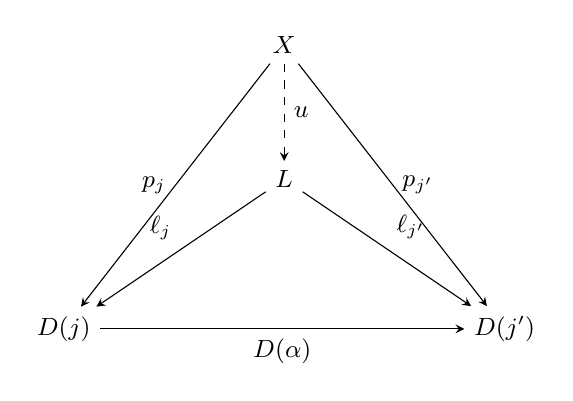
\begin{tikzpicture}[>=stealth,every node/.style={font=\small}]
 \node (x) at (0,3.6) {$X$};
 \node (l) at (0,1.9) {$L$};
 \node (j) at (-2.8,0) {$D(j)$};
 \node (k) at (2.8,0) {$D(j')$};
 \draw[->,dashed] (x) -- node[right] {$u$} (l);
 \draw[->] (x) -- node[left] {$p_j$} (j);
 \draw[->] (x) -- node[right] {$p_{j'}$} (k);
 \draw[->] (l) -- node[above left] {$\ell_j$} (j);
 \draw[->] (l) -- node[above right] {$\ell_{j'}$} (k);
 \draw[->] (j) -- node[below] {$D(\alpha)$} (k);
\end{tikzpicture}
\end{center}

Przekładając definicję: diagram to układ obiektów połączonych strzałkami; stożek to jeden obiekt z kompatybilnymi strzałkami do całego układu; granica jest \emph{najbardziej uniwersalnym} takim obiektem, ponieważ przez nią w jeden sposób przechodzą wszystkie inne stożki.

\begin{przyklad}[Iloczyn jako granica]
Niech $\mathcal J$ będzie dyskretną kategorią o dwóch obiektach, a $D(0)=A$, $D(1)=B$. Nie ma żadnych strzałek zgodności między różnymi obiektami. Stożek nad $D$ to dowolne dwa morfizmy $X\to A$ i $X\to B$, a uniwersalny stożek jest właśnie iloczynem $A\times B$ z definicji~\ref{def:produkt}. Dla rodziny indeksowanej zbiorem $I$ otrzymujemy w ten sposób iloczyn $\prod_{i\in I}A_i$.
\end{przyklad}

\begin{przyklad}[Equalizator jako granica]
Niech $\mathcal J$ ma dwa obiekty $0,1$ oraz dwa różne równoległe morfizmy $\alpha,\beta:0\to1$, oprócz identyczności. Wybór diagramu $D$ jest równoważny wyborowi pary $f,g:A\to B$. Stożek o wierzchołku $X$ ma strzałki $p_0:X\to A$ i $p_1:X\to B$ z $fp_0=p_1=gp_0$. Wszystkie dane poza $p_0$ są wymuszone, a warunek istnienia stożka to $fp_0=gp_0$. Granica jest więc equalizatorem $f$ i $g$.
\end{przyklad}

\begin{przyklad}[Granice w porządkach]
Dla kategorii posetu $(P,\leq)$ stożek o wierzchołku $x$ nad diagramem $D$ istnieje dokładnie wtedy, gdy $x\leq D(j)$ dla wszystkich $j$. Granica, jeśli istnieje, jest kresem dolnym zbioru wartości diagramu. Relacje między obiektami diagramu nie wnoszą tu dodatkowych równań, ponieważ odpowiednie hom-zbiory są co najwyżej jednoelementowe.
\end{przyklad}

\begin{twierdzenie}[Jednoznaczność granicy]\label{tw:limit-unique}
Jeśli dwa stożki $(L,(\ell_j)_j)$ i $(L',(\ell'_j)_j)$ są granicami tego samego diagramu $D$, to istnieje dokładnie jeden izomorfizm $u:L\to L'$ spełniający $\ell'_j\circ u=\ell_j$ dla wszystkich $j$.
\end{twierdzenie}
\begin{proof}
Z uniwersalności $(L',(\ell'_j)_j)$ zastosowanej do stożka o wierzchołku $L$ otrzymujemy jedyną strzałkę $u:L\to L'$ z $\ell'_ju=\ell_j$. Z uniwersalności $(L,(\ell_j)_j)$ zastosowanej do stożka o wierzchołku $L'$ otrzymujemy $v:L'\to L$ z $\ell_jv=\ell'_j$. Dla każdego $j$ mamy
\[
\ell_j(vu)=(\ell_jv)u=\ell'_ju=\ell_j=\ell_j\id_L.
\]
Zatem $vu$ i $\id_L$ faktoryzują ten sam stożek przez $L$. Jednoznaczność w definicji granicy daje $vu=\id_L$. Analogicznie
$\ell'_j(uv)=\ell_jv=\ell'_j=\ell'_j\id_{L'}$, skąd $uv=\id_{L'}$. Otrzymaliśmy izomorfizm, jedyny spośród morfizmów spełniających wymagane równania.
\end{proof}


\begin{twierdzenie}[Konstrukcja wszystkich małych granic w $\Set$]\label{tw:limits-set}
Niech $\mathcal J$ będzie małą kategorią i $D:\mathcal J\to\Set$ funktorem. Wówczas granica diagramu $D$ istnieje. Można ją zrealizować jako zbiór
\[
L=\left\{(x_j)_{j\in\Ob(\mathcal J)}\in\prod_{j\in\Ob(\mathcal J)}D(j):
D(\alpha)(x_j)=x_{j'}\ \text{dla każdego }\alpha:j\to j'\right\},
\]
z rzutami $\ell_j:L\to D(j)$, $\ell_j((x_i)_i)=x_j$.
\end{twierdzenie}
\begin{proof}
Rodzina rzutów jest stożkiem, ponieważ dla $\alpha:j\to j'$ oraz $x=(x_i)_i\in L$ z definicji mamy $D(\alpha)(\ell_j(x))=D(\alpha)(x_j)=x_{j'}=\ell_{j'}(x)$. Niech $X$ będzie dowolnym zbiorem ze stożkiem $p_j:X\to D(j)$. Zdefiniujmy $u:X\to\prod_jD(j)$ przez $u(x)=(p_j(x))_j$. Zgodność stożka daje $D(\alpha)(p_j(x))=p_{j'}(x)$, więc $u(x)\in L$. Dla każdego $j$ zachodzi $\ell_ju=p_j$. Jeśli $v:X\to L$ spełnia te same równości, to dla każdego $x\in X$ i każdego $j$ współrzędne $v(x)$ i $u(x)$ są równe. Zatem $u=v$. Otrzymaliśmy własność uniwersalną granicy, również gdy $\mathcal J$ jest pusta.
\end{proof}

\begin{przyklad}[Granica nad pustym diagramem i nad ciągiem stałym]
Jeżeli $\mathcal J$ nie ma obiektów, to iloczyn pustej rodziny zbiorów jest singletonem, a dodatkowe warunki nie występują. Granica pustego diagramu w $\Set$ jest więc jednoelementowa. Jeśli natomiast $X_n=\{0,1\}$ dla wszystkich $n$, a funkcje $p_n:X_{n+1}\to X_n$ są identycznościami, to granica odwrotna ma dokładnie dwa elementy: ciągi $(0,0,\ldots)$ oraz $(1,1,\ldots)$. Gdy wszystkie $p_n$ są stałe równe $0$, jedynym zgodnym ciągiem jest $(0,0,\ldots)$.
\end{przyklad}

\begin{przyklad}[Granice skończone w kategoriach przestrzeni liniowych]
Dla diagramu $D:\mathcal J\to\Vect_k$ o skończenie wielu obiektach i morfizmach definiujemy mapę liniową
\[
A:\prod_jD(j)\longrightarrow\prod_{\alpha:j\to j'}D(j'),
\qquad
A((x_j)_j)_\alpha=D(\alpha)x_j-x_{j'}.
\]
Jej jądro jest podprzestrzenią zgodnych krotek. Rzuty ograniczone do jądra są liniowe. Dla stożka liniowych map $p_j:X\to D(j)$ funkcja $x\mapsto(p_j(x))_j$ jest liniowa współrzędnie i przyjmuje wartości w $\Ker A$ dzięki równaniom stożka. Jednoznaczność wynika z jednoznaczności współrzędnych. Zatem $\Ker A$ wraz z rzutami jest granicą w $\Vect_k$. Konstrukcja z twierdzenia~\ref{tw:limits-set} nie jest przypadkowym trikiem zbiorowym: w algebrze liniowej sprowadza granice do układów równań liniowych.
\end{przyklad}


\subsection{Kogranica}

\begin{definicja}[Kostożek i kogranica]\label{def:colimit}
Dla diagramu $D:\mathcal J\to\mathcal C$ \emph{kostożek} o wierzchołku $X$ to rodzina $i_j:D(j)\to X$ spełniająca $i_{j'}\circ D(\alpha)=i_j$ dla każdego $\alpha:j\to j'$. \emph{Kogranicą} jest kostożek $(Q,(q_j)_j)$ taki, że każdy kostożek $(X,(i_j)_j)$ wyznacza dokładnie jeden $u:Q\to X$ spełniający $u\circ q_j=i_j$ dla wszystkich $j$. Oznaczamy $Q=\varinjlim_{j\in\mathcal J}D(j)$ lub $Q=\colim D$.
\end{definicja}
Dualnie dla każdego $\alpha:j\to j'$ otrzymujemy diagram kostożków z jednym wspólnym morfizmem $u$:
\begin{center}
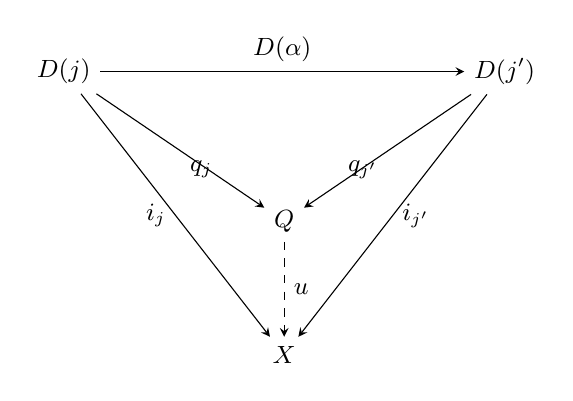
\begin{tikzpicture}[>=stealth,every node/.style={font=\small}]
 \node (j) at (-2.8,3.6) {$D(j)$};
 \node (k) at (2.8,3.6) {$D(j')$};
 \node (q) at (0,1.7) {$Q$};
 \node (x) at (0,0) {$X$};
 \draw[->] (j) -- node[above] {$D(\alpha)$} (k);
 \draw[->] (j) -- node[below right] {$q_j$} (q);
 \draw[->] (k) -- node[below left] {$q_{j'}$} (q);
 \draw[->] (j) -- node[left] {$i_j$} (x);
 \draw[->] (k) -- node[right] {$i_{j'}$} (x);
 \draw[->,dashed] (q) -- node[right] {$u$} (x);
\end{tikzpicture}
\end{center}

\begin{przyklad}[Koprodukt, koequalizator i pushout]
Koprodukt to kogranica diagramu dyskretnego. Koequalizator to kogranica diagramu dwóch równoległych strzałek. Pushout to kogranica diagramu $A\leftarrow C\to B$. Na odwrót, produkt, equalizator i pullback są odpowiednimi granicami. Formalne definicje tych sześciu pojęć to po prostu różne kształty tej samej własności uniwersalnej.
\end{przyklad}

\begin{przyklad}[Granica odwrotna ciągu zbiorów]\label{przyklad:inverse-limit}
Niech $X_0,X_1,X_2,\ldots$ będą zbiorami, a $p_n:X_{n+1}\to X_n$ funkcjami dla $n\geq0$. Granica odwrotna tego diagramu w $\Set$ jest zbiorem
\[
\varprojlim_{n\geq0}X_n=\{(x_0,x_1,\ldots)\in\prod_{n\geq0}X_n:p_n(x_{n+1})=x_n\text{ dla każdego }n\geq0\}.
\]
Zatem granica wybiera \emph{zgodne ciągi} elementów. Przykładowo dla $X_n=\mathbb Z/2^{n+1}\mathbb Z$ i redukcji modulo $2^{n+1}$ otrzymujemy zbiór $2$-adycznych liczb całkowitych $\mathbb Z_2$ (z odpowiednią strukturą pierścieniową).
\end{przyklad}

\begin{przyklad}[Kogranica rosnącego ciągu zbiorów]
Jeśli $X_0\subseteq X_1\subseteq\cdots$ i morfizmami są włączenia, to kogranicą w $\Set$ jest zwykła suma zbiorów $\bigcup_{n\geq0}X_n$. Jeżeli zamiast włączeń występują dowolne funkcje $X_n\to X_{n+1}$, odpowiednią kogranicę tworzymy z sumy rozłącznej wszystkich $X_n$, identyfikując element $x\in X_n$ z jego obrazem w $X_{n+1}$ i domykając te identyfikacje do relacji równoważności.
\end{przyklad}

\begin{przyklad}[Granice w rachunku liniowym]
W $\Vect_k$ granice skończonych diagramów można skonstruować za pomocą skończonych iloczynów i jąder, a kogranice za pomocą skończonych koproduktów i kojąder. Przykładowo dla $f:V\to W$ jądro $\Ker f$ to equalizator $f$ i zera; przestrzeń ilorazowa $W/\im f$ to ich koequalizator. Jest to początek języka kategorii addytywnych i abelowych.
\end{przyklad}

\begin{uwaga}[Ograniczenia wielkości]
Zakładamy, że $\mathcal J$ jest mała, więc wszystkie obiekty i strzałki diagramu są indeksowane zbiorami. W przeciwnym razie formuły typu $\prod_{j\in\Ob(\mathcal J)}D(j)$ mogą prowadzić do problemów teoriomnogościowych. Istnienie wszystkich \emph{małych} granic (odpowiednio kogranic) w kategorii nazywamy \emph{zupełnością} (odpowiednio \emph{kozupełnością}).
\end{uwaga}


\begin{twierdzenie}[Konstrukcja wszystkich małych kogranic w $\Set$]\label{tw:colimits-set}
Niech $\mathcal J$ będzie małą kategorią i $D:\mathcal J\to\Set$ diagramem. Zbudujmy sumę rozłączną $S=\coprod_{j\in\Ob(\mathcal J)}D(j)$, której elementy zapisujemy jako $(j,x)$ z $x\in D(j)$. Niech $\sim$ będzie najmniejszą relacją równoważności zawierającą pary
\[
(j,x)\sim(j',D(\alpha)(x))\quad \text{dla każdego }\alpha:j\to j'\text{ i }x\in D(j).
\]
Wówczas $Q=S/{\sim}$ wraz z mapami $q_j(x)=[(j,x)]$ jest kogranicą diagramu $D$.
\end{twierdzenie}
\begin{proof}
Dla $\alpha:j\to j'$ z definicji relacji mamy $q_{j'}(D(\alpha)(x))=[(j',D(\alpha)(x))]=[(j,x)]=q_j(x)$, więc $q_j$ tworzą kostożek. Niech $i_j:D(j)\to X$ będzie dowolnym kostożkiem. Funkcję $h:S\to X$ definiujemy na każdej składowej przez $h(j,x)=i_j(x)$. Warunek $i_{j'}D(\alpha)=i_j$ daje $h(j',D(\alpha)x)=h(j,x)$. Relacja $s\mathrel{R}t$ wtedy i tylko wtedy, gdy $h(s)=h(t)$, jest relacją równoważności zawierającą wszystkie generatory $\sim$. Z minimalności $\sim$ wynika $\sim\,\subseteq R$, czyli $h$ jest stała na klasach $\sim$. Zatem istnieje jednoznaczna funkcja $\bar h:Q\to X$, $\bar h([(j,x)])=i_j(x)$, i spełnia ona $\bar hq_j=i_j$. Jedyność wynika z tego, że każdy element $Q$ jest klasą pewnego $(j,x)$; wartości na obrazach wszystkich $q_j$ wyznaczają więc całą funkcję. Dla pustego $\mathcal J$ otrzymujemy $Q=\varnothing$.
\end{proof}

\begin{przyklad}[Kogranica diagramu, który scala dwa punkty]
Niech $X_n=\{0,1\}$ dla $n\geq0$, a wszystkie mapy $f_n:X_n\to X_{n+1}$ będą stałe i równe $0$. W kogranicy elementy $(n,0)$ oraz $(n,1)$ są utożsamione, gdyż oba przechodzą do $(n+1,0)$. Wszystkie elementy całej sumy rozłącznej należą do jednej klasy, więc kogranica jest singletonem. Gdy zamiast tego wszystkie $f_n$ są identycznościami, pozostają dokładnie dwie klasy, odpowiadające $0$ i $1$.
\end{przyklad}

\begin{przyklad}[Liczby $2$-adyczne jako zgodne reszty]
W przykładzie~\ref{przyklad:inverse-limit} weźmy układ reszt modulo $2,4,8,16,\ldots$. Ciąg $([1]_2,[3]_4,[7]_8,[15]_{16},\ldots)$ jest zgodny, ponieważ $2^{n+2}-1$ redukuje się modulo $2^{n+1}$ do $2^{n+1}-1$. Reprezentuje on liczbę $-1$ w pierścieniu $\mathbb Z_2$. Natomiast ciąg $([0]_2,[1]_4,\ldots)$ nie jest zgodny: $[1]_4$ po redukcji modulo $2$ daje $[1]_2$, a nie $[0]_2$. Ten prosty rachunek wyjaśnia, jakie dane dopuszcza granica odwrotna.
\end{przyklad}

\subsection{Istnienie granic i kogranic w ogólnych kategoriach}

\begin{twierdzenie}[Iloczyny i equalizatory wystarczają]\label{cat:thm:limits-products}
Jeżeli kategoria $\mathcal C$ ma wszystkie małe iloczyny i equalizatory, to ma wszystkie małe granice. Wystarczy istnienie skończonych iloczynów (w tym pustego) i equalizatorów, aby istniały granice wszystkich skończonych kategorii indeksujących. Dualnie, małe koprodukty i koequalizatory zapewniają wszystkie małe kogranice; wersja skończona również zachodzi.
\end{twierdzenie}
\begin{proof}
Dla diagramu $D:\mathcal J\to\mathcal C$ tworzymy
$P=\prod_jD(j)$ oraz $R=\prod_{\alpha:j\to j'}D(j')$.
Niech $s,t:P\to R$ będą wyznaczone przez składowe
$\pi_\alpha s=D(\alpha)\pi_j$ oraz $\pi_\alpha t=\pi_{j'}$.
Jeśli $e:L\to P$ jest equalizatorem $s,t$, to $\pi_je$ tworzą stożek. Dowolny stożek $(p_j:X\to D(j))$ wyznacza jedyną mapę $p:X\to P$. Równości stożka są równoważne $sp=tp$, więc istnieje jedyna $u:X\to L$ z $eu=p$. Jedyność mapy do iloczynu zapewnia, że warunki $\pi_jeu=p_j$ są równoważne $eu=p$. To dowodzi własności granicy. Dla kogranicy bierzemy $S=\coprod_jD(j)$ i $U=\coprod_{\alpha:j\to j'}D(j)$. Oznaczmy włączenia przez $i_j:D(j)\to S$ oraz $k_\alpha:D(j)\to U$. Definiujemy $r,t:U\to S$ przez $rk_\alpha=i_j$ oraz $tk_\alpha=i_{j'}D(\alpha)$. Jeśli $q:S\to Q$ jest ich koequalizatorem, to $qi_j=qrk_\alpha=qtk_\alpha=qi_{j'}D(\alpha)$, więc $qi_j$ tworzą kostożek. Dowolny kostożek $(h_j:D(j)\to X)$ wyznacza jedyną mapę $h:S\to X$ z $hi_j=h_j$. Zgodność kostożka daje $hrk_\alpha=htk_\alpha$ dla wszystkich $\alpha$, a z własności koproduktu $U$ wynika $hr=ht$. Koequalizator daje jedyną mapę $v:Q\to X$ z $vq=h$. Warunek ten jest równoważny $vqi_j=h_j$ dla wszystkich $j$, z jednoznaczności mapy z koproduktu $S$. To dowodzi istnienia i jednoznaczności faktoryzacji również dla pustego diagramu.
\end{proof}

\begin{uwaga}
Odwrotność jest natychmiastowa: iloczyny i equalizatory są szczególnymi granicami. Granica pustego diagramu to obiekt końcowy, a kogranica pustego diagramu to obiekt początkowy, o ile istnieją.
\end{uwaga}

\subsection{Granice punktowe i iterowane}

\begin{twierdzenie}[Granice i kogranice funktorów]\label{cat:thm:pointwise-limits}
Niech $\mathcal A$ będzie małą kategorią, $\mathcal J$ małą kategorią indeksującą, a $F:\mathcal J\to[\mathcal A,\mathcal C]$ diagramem funktorów, gdzie $\mathcal C$ jest lokalnie mała. Jeśli dla każdego $a$ istnieje granica diagramu $j\mapsto F(j)(a)$, to granica $F$ istnieje w kategorii funktorów i jest obliczana punktowo. Dualnie dla kogranic.
\end{twierdzenie}
\begin{proof}
Wybierzmy granice $L(a)$ z rzutami $\ell_{j,a}$. Dla $f:a\to b$ oraz $\alpha:j\to k$ naturalność $F(\alpha)$ i zgodność stożka dają
\[
F(\alpha)_bF(j)(f)\ell_{j,a}
=F(k)(f)F(\alpha)_a\ell_{j,a}
=F(k)(f)\ell_{k,a}.
\]
Zatem strzałki $F(j)(f)\ell_{j,a}$ tworzą stożek nad diagramem w $b$. Jedyna mapa $L(f):L(a)\to L(b)$ spełnia
$\ell_{j,b}L(f)=F(j)(f)\ell_{j,a}$.
Dla identyczności mamy $\ell_{j,a}L(\id_a)=\ell_{j,a}$, więc $L(\id_a)=\id_{L(a)}$. Dla $g:b\to c$ zachodzi
\[
\ell_{j,c}L(g)L(f)=F(j)(g)F(j)(f)\ell_{j,a}
=F(j)(gf)\ell_{j,a}=\ell_{j,c}L(gf).
\]
Jednoznaczność w granicy $L(c)$ daje $L(g)L(f)=L(gf)$. Równania definiujące $L(f)$ są naturalnością rzutów $\ell_j:L\to F(j)$. Stożek $(p_j:H\to F(j))_j$ wyznacza punktowo jedyne mapy $u_a:H(a)\to L(a)$ z $\ell_{j,a}u_a=p_{j,a}$. Dla $f:a\to b$ obliczamy
\[
\ell_{j,b}L(f)u_a=F(j)(f)p_{j,a}
=p_{j,b}H(f)=\ell_{j,b}u_bH(f).
\]
Z jednoznaczności w $L(b)$ otrzymujemy $L(f)u_a=u_bH(f)$. Rodzina $u_a$ jest więc transformacją naturalną i jedynym morfizmem stożków. Dla kogranic stosujemy argument do diagramu $\mathcal J^{\op}\to[\mathcal A^{\op},\mathcal C^{\op}]$, otrzymanego przez odwrócenie strzałek i transformacji naturalnych. Odwrócenie wyniku daje dokładnie kostożek i jego własność uniwersalną w $[\mathcal A,\mathcal C]$.
\end{proof}

\begin{twierdzenie}[Iterowanie granic tego samego rodzaju]\label{cat:thm:iterated-limits}
Dla diagramu $D:\mathcal I\times\mathcal J\to\mathcal C$ w kategorii zupełnej, przy małych $\mathcal I,\mathcal J$, istnieją kanoniczne izomorfizmy
\[
\lim_i\lim_jD(i,j)\cong\lim_{(i,j)}D(i,j)
\cong\lim_j\lim_iD(i,j).
\]
W kategorii kozupełnej zachodzi dualne twierdzenie dla dwóch kogranic.
\end{twierdzenie}
\begin{proof}
Dla każdego $i$ wybierzmy granicę $L_i=\lim_jD(i,j)$ i rzuty $r_{i,j}:L_i\to D(i,j)$. Jeśli $\alpha:i\to i'$ oraz $\beta:j\to j'$, to funktorialność $D$ daje
\[
D(\id_{i'},\beta)D(\alpha,\id_j)
=D(\alpha,\id_{j'})D(\id_i,\beta).
\]
Po złożeniu z $r_{i,j}$ prawa strona jest równa $D(\alpha,\id_{j'})r_{i,j'}$. Rodzina $D(\alpha,\id_j)r_{i,j}$ jest więc stożkiem, co wyznacza jedyną strzałkę $L(\alpha):L_i\to L_{i'}$ taką, że
\[
r_{i',j}L(\alpha)=D(\alpha,\id_j)r_{i,j}.
\]
Dla identyczności równania te spełnia identyczność $L_i$, a dla złożenia dwóch strzałek spełnia je złożenie odpowiednich map $L(\alpha)$. Jednoznaczność zapewnia zatem funktorialność $L$.

Niech $M=\lim_iL_i$ z rzutami $m_i:M\to L_i$. Rodzina $r_{i,j}m_i$ jest zgodna w kierunku $j$ dzięki stożkom $r_{i,j}$, a w kierunku $i$, ponieważ
\[
D(\alpha,\id_j)r_{i,j}m_i
=r_{i',j}L(\alpha)m_i=r_{i',j}m_{i'}.
\]
Każda strzałka $(\alpha,\beta)$ jest złożeniem strzałek w tych dwóch kierunkach; rodzina jest więc stożkiem nad $D$.

Niech teraz $p_{i,j}:X\to D(i,j)$ będzie dowolnym stożkiem. Dla ustalonego $i$ istnieje jedyna $v_i:X\to L_i$ z $r_{i,j}v_i=p_{i,j}$. Zgodność w kierunku $i$ daje
\[
r_{i',j}L(\alpha)v_i
=D(\alpha,\id_j)p_{i,j}=p_{i',j}=r_{i',j}v_{i'}.
\]
Jednoznaczność w granicy $L_{i'}$ daje $L(\alpha)v_i=v_{i'}$. Istnieje zatem jedyna $u:X\to M$ z $m_iu=v_i$; spełnia ona $r_{i,j}m_iu=p_{i,j}$. Jeśli $w:X\to M$ spełnia te same równania, najpierw jednoznaczność w $L_i$ daje $m_iw=v_i$ dla każdego $i$, a następnie jednoznaczność w $M$ daje $w=u$. Jest to własność granicy $D$.

Po zamianie $\mathcal I$ i $\mathcal J$ dostajemy drugi stożek graniczny, więc twierdzenie~\ref{tw:limit-unique} daje oba izomorfizmy zgodne z rzutami. Dla kogranic stosujemy udowodniony wynik do $D^{\op}:\mathcal I^{\op}\times\mathcal J^{\op}\to\mathcal C^{\op}$: granice w kategorii przeciwnej są dokładnie kogranicami w wyjściowej, z odwróconymi morfizmami stożków.
\end{proof}

\begin{przyklad}[Punktowe granice reprezentowalnych funktorów]
Jeśli $L$ jest granicą diagramu $D$ w lokalnie małej kategorii, to dla każdego $X$ zbiór $\Hom(X,L)$ jest naturalnie izomorficzny z $\lim_j\Hom(X,D(j))$: bijekcja przypisuje $u$ rodzinę $(\ell_ju)_j$, a naturalność w $X$ wynika z prekompozycji. Dualnie $\Hom(Q,X)\cong\lim_j\Hom(D(j),X)$ dla kogranicy $Q$, gdzie po prawej indeksujemy przez $\mathcal J^{\op}$.
\end{przyklad}

\subsection{Kogranice filtrowane}

\begin{definicja}[Kategoria filtrowana]\label{cat:def:filtered}
Mała kategoria $\mathcal J$ jest filtrowana, jeśli jest niepusta, każde dwa obiekty mają strzałki do wspólnego obiektu, a każda para równoległych strzałek $f,g:i\to j$ ma strzałkę $h:j\to k$ z $hf=hg$. Przykładem jest niepusty porządek skierowany, w szczególności $\mathbb N$ z naturalnym porządkiem.
\end{definicja}

\begin{lemat}[Równość reprezentantów]\label{cat:lem:filtered-equality}
Dla diagramu zbiorów $D$ o małej filtrowanej kategorii indeksującej klasy $[(i,x)]$ i $[(j,y)]$ w kogranicy są równe wtedy i tylko wtedy, gdy istnieją strzałki $i\to k$, $j\to k$, po których obrazy $x,y$ są równe.
\end{lemat}
\begin{proof}
Najpierw pokażemy, że dla skończonej listy obiektów i strzałek między nimi można znaleźć obiekt $k$ i mapy $b_i:i\to k$ zgodne z każdą z wymienionych strzałek. Dla listy pustej wybieramy dowolny obiekt (niepustość). Dla listy niepustej stosujemy kolejno drugi aksjomat filtrowania, składając dotychczasowe mapy z mapą do nowego wspólnego obiektu. Otrzymujemy mapy $b_i:i\to k$, początkowo bez warunków zgodności.

Dla strzałki $\alpha:i\to j$ porównujemy równoległe mapy $b_i,b_j\alpha:i\to k$. Trzeci aksjomat daje $h:k\to k'$ z $hb_i=hb_j\alpha$. Zastępujemy wszystkie $b_l$ przez $hb_l$. Równania już uzyskane pozostają prawdziwe po złożeniu z $h$. Po skończenie wielu takich krokach wszystkie wymagane równania są spełnione.

Najmniejsza relacja równoważności z twierdzenia~\ref{tw:colimits-set} składa się dokładnie z par połączonych skończonym ciągiem identyfikacji generujących, ich odwróceń lub równości. Istotnie, relacja opisana przez takie ciągi jest zwrotna (ciąg pusty), symetryczna (odwrócenie ciągu) i przechodnia (konkatenacja ciągów), a każda relacja równoważności zawierająca generatory musi ją zawierać.

Jeżeli $[(i,x)]=[(j,y)]$, wybierzmy taki ciąg. Zastosujmy pierwszą część dowodu do wszystkich obiektów i strzałek użytych w tym ciągu. Każda identyfikacja $(l,z)\sim(l',D(\alpha)z)$ ma po przeniesieniu do $k$ równe obrazy, gdyż
\[
D(b_{l'})D(\alpha)z=D(b_{l'}\alpha)z=D(b_l)z.
\]
Równość zachodzi także dla identyfikacji odwróconych. Przechodniość równości daje $D(b_i)x=D(b_j)y$.

Odwrotnie, jeżeli dla $b:i\to k$ oraz $c:j\to k$ zachodzi $D(b)x=D(c)y$, to $(i,x)\sim(k,D(b)x)=(k,D(c)y)\sim(j,y)$.
\end{proof}

\begin{twierdzenie}[Kogranice filtrowane a granice skończone w $\Set$]\label{cat:thm:filtered-finite}
W kategorii zbiorów kogranice filtrowane komutują z granicami skończonych diagramów: dla małej filtrowanej $\mathcal J$, skończonej $\mathcal I$ i $D:\mathcal J\times\mathcal I\to\Set$ kanoniczna mapa
\[
\colim_j\lim_i D(j,i)\longrightarrow
\lim_i\colim_j D(j,i)
\]
jest bijekcją.
\end{twierdzenie}
\begin{proof}
Dla każdego $j$ oznaczmy przez $L_j=\lim_iD(j,i)$ zbiór zgodnych krotek. Morfizm $j\to k$ działa współrzędnie na krotkach, ponieważ $D$ jest funktorem na kategorii produktowej. Kanoniczna funkcja
\[
\Phi:\colim_j L_j\longrightarrow\lim_i\colim_jD(j,i)
\]
przypisuje klasie $[(j,(x_i)_i)]$ krotkę $([(j,x_i)])_i$. Jest dobrze określona: identyfikacja w kogranicy po lewej daje identyfikacje współrzędnych po prawej, a zgodność krotki w $L_j$ daje zgodność jej klas.

\emph{Surjektywność.} Weźmy zgodną rodzinę klas $(c_i)_i$ po prawej. Wybierzmy reprezentanty $c_i=[(j_i,x_i)]$. Obiektów $i$ jest skończenie wiele, zatem istnieje wspólny etap $j$ oraz strzałki $j_i\to j$. Po przeniesieniu reprezentantów mamy $c_i=[(j,y_i)]$. Jeżeli $\beta:i\to i'$ jest strzałką w $\mathcal I$, zgodność klas oznacza
\[
[(j,D(j,\beta)y_i)]=[(j,y_{i'})].
\]
Lemat~\ref{cat:lem:filtered-equality} daje dwie strzałki z $j$ do pewnego $k_\beta$, po których obrazy tych elementów są równe. Wyrównujemy te dwie strzałki trzecim aksjomatem filtrowania, otrzymując jedną strzałkę $a_\beta:j\to k'_\beta$, po której obrazy są równe. Ponieważ strzałek $\beta$ jest skończenie wiele, stosujemy konstrukcję z dowodu lematu do układu wszystkich $a_\beta$, otrzymując jedną strzałkę $a:j\to k$ faktoryzującą każdą z nich. Jeśli strzałek nie ma, bierzemy dowolny wspólny etap (można wziąć $j$). Definiujemy $z_i=D(a,i)y_i$. Dla każdej $\beta:i\to i'$ funktorialność daje
\[
D(k,\beta)z_i=D(a,i')D(j,\beta)y_i=D(a,i')y_{i'}=z_{i'}.
\]
Stąd $(z_i)_i\in L_k$ i $\Phi([(k,(z_i)_i)])=(c_i)_i$.

\emph{Injektywność.} Niech obrazy klas reprezentowanych przez $(x_i)_i\in L_j$ oraz $(y_i)_i\in L_{j'}$ będą równe. Dla każdej współrzędnej lemat daje etap $k_i$ oraz strzałki $b_i:j\to k_i$, $c_i:j'\to k_i$, po których obrazy $x_i,y_i$ są równe. Skończony układ tych strzałek ma zgodny kostożek do pewnego $k$ (konstrukcja z dowodu lematu). Otrzymujemy więc dwie strzałki $b:j\to k$, $c:j'\to k$ faktoryzujące odpowiednio wszystkie $b_i,c_i$. Obrazy krotek są równe we wszystkich współrzędnych, czyli są równe w $L_k$. Lemat zastosowany do diagramu $j\mapsto L_j$ daje równość klas po lewej.

Dla pustej $\mathcal I$ każdy $L_j$ jest singletonem, podobnie granica po prawej. Kogranica stałego singletonu jest singletonem, bo $\mathcal J$ jest niepusta, a każde dwa obiekty mają wspólny etap. Tym samym uwzględniono również granicę pustą.
\end{proof}

\begin{przyklad}[Dlaczego skończoność jest istotna]\label{cat:ex:filtered-infinite}
Niech $A_n=\{0,\ldots,n\}$ z włączeniami i niech indeks współrzędnych przebiega $\mathbb N$. Mapa
$\colim_n A_n^{\mathbb N}\to(\colim_n A_n)^{\mathbb N}=\mathbb N^{\mathbb N}$
jest włączeniem ciągów ograniczonych w zbiór wszystkich ciągów. Ciąg $a_k=k$ nie należy do obrazu. Kogranica filtrowana nie musi więc komutować z nieskończonym iloczynem.
\end{przyklad}

\subsection{Granice odwrotne w topologii i algebrze}

\begin{przyklad}[Solenoid]
Dla liczby całkowitej $p\ge2$ weźmy okręgi $S^1$ i mapy $z\mapsto z^p$. Ich granica odwrotna w $\Top$ jest podprzestrzenią produktu $(S^1)^{\mathbb N}$ złożoną z ciągów spełniających $z_n=z_{n+1}^p$. Rzuty są ciągłe, a mapa do produktu jest ciągła dokładnie wtedy, gdy wszystkie jej składowe są ciągłe; to dowodzi własności uniwersalnej z topologią podprzestrzeni. Tak otrzymuje się solenoid, omawiany szerzej w \atlasref{TOP-10::thm:solenoid-v4}{TOP-10: homologia i kohomologia Čecha solenoidu}.
\end{przyklad}

\begin{przyklad}[Granica odwrotna nie zachowuje epimorfizmów]\label{cat:ex:inverse-not-exact}
Dla $n\ge1$ rozważmy zgodne krótkie ciągi dokładne grup abelowych
$0\to2^n\mathbb Z\to\mathbb Z\to\mathbb Z/2^n\mathbb Z\to0$.
Mapami przejścia są włączenia po lewej, identyczności pośrodku i redukcje po prawej. Granice tych trzech układów wynoszą odpowiednio $0$, $\mathbb Z$, $\mathbb Z_2$. Mapa $\mathbb Z\to\mathbb Z_2$ nie jest surjektywna: wybór dowolnego nieskończonego ciągu cyfr binarnych daje zgodne reszty, różne ciągi dają różne elementy, więc $\mathbb Z_2$ jest nieprzeliczalny, a $\mathbb Z$ przeliczalny. Granice w $\Ab$ obliczamy jako podgrupy produktu zgodnych krotek, zatem przykład pokazuje brak prawostronnej dokładności granicy odwrotnej. Jest to adaptacja \atlasref{TOP-10::prz:cech-lim-niedokladnosc}{TOP-10: przykładu niedokładności granicy odwrotnej}.
\end{przyklad}

\begin{uwaga}[Pierwsza przeszkoda: $\lim^1$]\label{cat:rem:lim-one}
Dla przeliczalnego układu odwrotnego grup abelowych $(A_n,u_n)$ kładziemy $T((a_n)_n)=(u_n(a_{n+1}))_n$. Wtedy
\[
\lim_n A_n=\Ker(1-T),\qquad
\lim\nolimits^1_n A_n=\operatorname{coker}(1-T)
\]
na produkcie $\prod_n A_n$. Pierwsza równość to równania zgodności; druga jest standardowym opisem pierwszego pochodnego funktora granicy dla takich układów (AT-29). Jeśli wszystkie $u_n$ są surjektywne, to $1-T$ jest surjektywne: dla zadanego $(b_n)$ wybieramy $a_0=0$, a następnie $a_{n+1}$ z $u_n(a_{n+1})=a_n-b_n$. Stąd $\lim^1 A_n=0$. Ogólnie wystarcza warunek Mittaga--Lefflera, czyli stabilizacja obrazów $A_m\to A_n$ dla każdego ustalonego $n$; dowód podano w \atlasref{TOP-29::thm:xviii-ml}{TOP-29: warunek Mittaga--Lefflera dla układów przeliczalnych}. Nie należy utożsamiać zwykłej granicy z granicą homotopijną ani automatycznie przenosić tej formuły na dowolne kategorie indeksujące.
\end{uwaga}
